\chapter{Electroosmosis in a finite cylindrical pore: simple models of end effects}\label{chpt:finite_thickness}
\newcommand*\mycommand[1]{\texttt{\emph{#1}}}
\section{Introduction}
A theoretical model of electroosmosis through a circular pore of radius $a$ that traverses a membrane of thickness $h$ is investigated. Both the cylindrical surface of the pore and the outer surfaces of the membrane are charged. Electroosmosis in a circular cylindrical pore of finite length $h$ differs from that in an infinitely long pore due to end effects. If the cylinder length $h=0$, the pore consists of a hole in a charged membrane of zero thickness, and electroosmosis can be considered to be entirely due to end effects. This case was considered by us previously \cite{mao2014} and details given in Chapter \ref{chpt:zero_thickness}. When the cylindrical pore is infinitely long, end effects are negligible, and the computation of the electroosmotic volumetric flow rate $Q$, for arbitrary Debye lengths and surface charge densities, is standard \cite{rice1965,gross1968}
(with similar results available for infinitely long planar channels \cite{baldessari2008a,baldessari2008b}). Here we are interested in intermediate values of $h$. 

Full numerical computation of the Poisson-Nernst-Planck (PNP) equations for ionic motion is of course possible, and some typical results were reported by Mao et al. \cite{mao2014}. Such numerical computations, however, do not identify the mechanisms underlying the qualitative features of the physical system. Here we discuss how simple models, based upon continuity of electric current and volumetric flow rate, can be combined in order to estimate end effects for pore lengths $h>0$. We assume that the zeta potential on the surface of the membrane is small, so that the Poisson-Boltzmann equation governing the equilibrium charge cloud can be linearized, and the electroosmotic velocity can be determined by an analysis equivalent to that of Henry \cite{Henry_1931} for electrophoresis, i.e. fluid motion is generated by the effect of the applied electric field acting on the equilibrium charge cloud (which is not deformed either by the applied electric field or by fluid motion). In this limit the electroosmotic volumetric flow rate $Q$ through the hole in
the membrane can be determined by means of the reciprocal theorem \cite{mao2014}.

\begin{figure}[ht]
\centering
\includegraphics[width=0.8\textwidth]{finite_thickness/finite_pore_pic1.eps}
\caption{The cylindrical pore CD, of length $h$ and radius $a$ with surface charge density $\sigma_c$, passing through the membrane with surface charge density $\sigma_m$ on the two surfaces BC and DE. The reservoirs on either side of the membrane are large ($b\gg a$). The pore and reservoirs are axisymmetric about the $z$ axis.}
\label{Fig:schematic}
\end{figure}

Figure \ref{Fig:schematic} shows the axisymmetric geometry that we are considering. The cylindrical pore CD has radius $a$ and length $h$.
The cylindrical surface CD of the pore has surface charge density $\sigma_c$, and the membrane surfaces BC and DE have surface charge density $\sigma_m$. An electrical potential difference is applied betwen the fluid reservoirs at either side of the membrane, and electroosmotic flow is generated by the resulting electric field acting on the charge cloud adjacent to the charged surfaces.
The analysis of Mao et al. \cite{mao2014} assumed that the external reservoirs on either side of the pore were unbounded, with radius $b=\infty$. For the numerical computations presented in section \ref{sec:finite_numerical}, the external reservoirs were bounded by uncharged cylinders of radius $b\gg a$,  sufficiently large that numerical results when $h=0$ differed little from the analytic results for $h=0$ and $b$ infinite.  There have been many studies in which flow is generated in cylinders of different dimensions, connected either in series \cite{biscombe2012} or in networks intended to represent porous media \cite{jin1991}. Here, however, we are interested in the effect of the surfaces BC and DE of the membrane on electroosmotic flow within the cylindrical pore, and any boundaries AB, EF of the external reservoirs are so far away that they can be neglected.

We shall allow the surface charge density $\sigma_m$ on the membrane to differ from the charge density $\sigma_c$ on the wall of the cylindrical pore. There have been previous detailed studies of the effect of a discontinuity in surface charge density on electroosmosis \cite{yariv2004,khair2008}. The fine details of the charge cloud and fluid motion around such a discontinuity will be lost by the simple models presented here. They are, of course, fully taken into account in the numerical computations discussed in section \ref{sec:finite_numerical}.

In section \ref{subsec:finite_composite} we set up the approximate analysis of end effects, and compare results to those obtained from full numerical computations. The analysis is presented from first principles, but can alternatively be set within the framework of the reciprocal theorem, as explained in section \ref{subsec:finite_composite1}. The agreement between the approximate analysis and full computation is in general good, except for large Debye lengths $\kappa^{-1}\gg a$. In section \ref{sec:finite_overspill} we consider this case in more detail, in order to evaluate how much of the charge cloud due to the charged walls of the cylindrical pore lies within the pore and how much spills out beyond the ends of the pore. When this overspill is taken into account, the agreement between the computations and the approximate model is improved.

\section{Composite electroosmotic coefficient}
\subsection{The pore geometry}
The axisymmetric geometry that we are considering is shown in Figure \ref{Fig:schematic}. We use cylindrical polar coordinates $(r,z)$, with the $z$ axis along the axis of symmetry and $z=0$ at the midpoint of the cylindrical pore, the ends of which are at $z=\pm h/2$. When $h=0$ we shall also use oblate spherical coordinates $(\xi,\eta)$, with
\begin{equation}
z=a\sinh\xi\cos\eta\quad,\quad r=a\cosh\xi\sin\eta,
\end{equation}
where $-\infty<\xi<\infty$ and $0\le \eta<\pi/2$.

The cylindrical pore and the reservoirs at either end are filled with liquid with electrical conductivity $\Sigma$ and viscosity $\mu$. The wall CD of the cylindrical pore is charged, with uniform surface charge density $\sigma_c$, and the surface charge density
over the membrane surfaces BC, DE, is $\sigma_m$. The electrical permittivity $\epsilon_s$ of the membrane will be typically much
smaller than the permittivity $\epsilon$ of the liquid, and we assume $\epsilon_s=0$. We assume that the reservoir boundaries AB, EF are uncharged and at infinity. We shall occasionally refer to the surface potential $\zeta$, which will not in general be uniform, but which is required to be small, with $\zeta\ll kT/e$, where $e$ is the elementary charge and $kT$ the Boltzmann temperature. The electrical potential $\phi_0$ within the equilibrium charge cloud therefore satisfies the linearized Poisson-Boltzmann equation, so that
\begin{equation}
\nabla^2\phi_0=\kappa^2\phi_0,
\label{eq:linear_poisson_boltzmann_eqn}
\end{equation}
where $\kappa^{-1}$ is the Debye length, and the charge density in the equilibrium charge cloud is
\begin{equation}
\rho_0=-\epsilon\kappa^2\phi_0.
\end{equation}

\subsection{The applied electric field}
\label{subsec:finite_composite}
The applied electric field is
$\mathbf{E}=-\nabla\chi$,
where the potential $\chi$ satisfies the Laplace equation
\begin{equation}
\nabla^2\chi=0,
\end{equation}
with gradient
\begin{equation}
\mathbf{n} \cdot \nabla\chi=0
\end{equation}
normal to the walls of the membrane and of the cylindrical pore. In $z>0$, the electric potential far from the membrane is $\chi=\phi_1/2$, and the potential far from the membrane in $z<0$ is $\chi=-\phi_1/2$.

When the membrane thickness $h=0$, the potential can be expressed explicitly as \cite{M&F}
\begin{equation}
\chi=\frac{\phi_1}{2}\left\lbrack 1-\frac{2}{\pi}
\tan^{-1}\left(\frac{1}{\sinh\xi}\right)\right\rbrack
=\tilde\chi_m(r,z)\phi_1.
\label{chi_m}
\end{equation}
On the plane of the membrane, within the circular opening,
\begin{equation}
\tilde\chi_m=0,\hskip 20pt z=0,\ r<a,\ h=0.
\label{chi_m_z0}
\end{equation}

The liquid within the pore has electrical conductivity $\Sigma$; we have assumed that surface charge density (and hence the density of charge in the cloud of counter ions) is small, so that surface conductivity may be neglected. Indeed, if the mobilities of the various ionic species are identical, the surface conductivity due to the mobile charge cloud given by the linearized model (Equation \ref{eq:linear_poisson_boltzmann_eqn}) at $O(e\zeta/kT)$ is zero. The total electric current $I_m$ flowing through the hole in the membrane is therefore
\begin{equation}
I_m=-\frac{\phi_1}{R_m}\quad,\quad R_m=\frac{1}{2a\Sigma}.
\label{Im_h0}
\end{equation}

If $h>0$, we assume that the potential within the cylindrical pore varies linearly and approximate the potential within the pore as
\begin{equation}
\chi=\tilde\chi_c\phi_2=\frac{z}{h}\phi_2,\hskip 20pt r<a,\ |z|<h/2,
\label{approx_chi_c}
\end{equation}
as would be expected in the absence of any end effects. The potential in $z>h/2$ is approximated by that outside a membrane (with a hole) of zero thickness:
\begin{equation}
\chi=\frac{\phi_2}{2}+(\phi_1-\phi_2)\tilde\chi_m(r,z-h/2),
\label{approx_chi_m}
\end{equation}
with $\chi(r,z)=-\chi(r,-z)$. This approximation (Equation \ref{approx_chi_c} and \ref{approx_chi_m}) is continuous at $z=\pm h/2$ where the potential is assumed to be $\pm \phi_2/2$ across the entire width of the opening (by Equation \ref{chi_m_z0}). The as yet unspecified
potential $\phi_2$ is determined by requiring continuity of the electrical current at $z=\pm h/2$. The current $I_c$ through the cylindrical pore is
\begin{equation}
I_c=-\frac{\phi_2}{R_c}\quad,\quad R_c=\frac{h}{\pi a^2\Sigma},
\label{I_c}
\end{equation}
and the electrical current through the reservoir in $z>h/2$ is, by Equation \ref{Im_h0},
\begin{equation}
I_m=- \frac{\phi_1-\phi_2}{R_m}.
\label{I_m}
\end{equation}
Equating $I_c$ (Equation \ref{I_c}) and  $I_m$ (Equation \ref{I_m}), we find
\begin{equation}
\phi_2=\frac{R_c\phi_1}{R_m+R_c}.
\label{phi_2}
\end{equation}
This computation suggests that the system can be treated as two resistors in series, with composite resistance
\begin{equation}
R_\text{comp}=R_m+R_c.
\label{R_comp_defn}
\end{equation}
However, this estimate assumes a uniform potential over the ends of the pore at $z=\pm h/2$, and we have effectively inserted thin, perfectly conducting sheets over the pore ends. Removal of these sheets can only increase the resistance, and hence $R_\text{comp}$ is an underestimate for the true total resistance $R_\text{tot}$. Figure \ref{Fig:Rcomp}(a) shows $R_\text{tot}/(a\Sigma)$ computed numerically by means of the Freefem++ finite element package \cite{hecht2012}, together with $R_\text{comp}/(a\Sigma)$. The difference is small, and is shown in Figure \ref{Fig:Rcomp}(b).

\begin{figure}[ht]
\begin{center}
\includegraphics[width=\textwidth]{finite_thickness/finite_pore_pic6.eps}
\end{center}
\caption{(a) The non-dimensional Ohmic resisistance $R/(a\Sigma)$ of a hole of radius $a$ in a membrane of thickness $h$, as a function of
$h/a$. Solid line, $R_{tot}/(a\Sigma)$ computed numerically; dashed line, the approximation $R_{comp}/(a\Sigma)$ Equation (\ref{R_comp_defn}). (b) The difference $(R_{tot}-R_{comp})/(a\Sigma)$.}
\label{Fig:Rcomp}
\end{figure}

\subsection{Electroosmosis through an infinite cylindrical pore}
We assume throughout this paper that the perturbation of the equilibrium charge cloud by the applied electric field and by fluid motion is negligibly small. The force acting on the ions in the charge cloud due to the applied electric field $-\nabla\chi$ is therefore $-\rho_0\nabla\chi$.

The equilibrium potential within an infinite cylindrical pore is
\begin{equation}
\phi_0=\zeta_c\frac{I_0(\kappa r)}{I_0(\kappa a)}
=\frac{\sigma_c}{\epsilon\kappa}\frac{I_0(\kappa r)}{I_1(\kappa a)}.
\label{phi0_cylinder}
\end{equation}
In the absence of any end effects, if the electric field $E_0=-\phi_2/h$ is applied along the length of the cylindrical pore, the fluid velocity is \cite{levine1975}
\begin{equation}
u=\frac{\epsilon\phi_2}{\mu h}(\zeta_c-\phi_0),
\end{equation}
and the total electroosmotic volumetric flow rate is \cite{rice1965}
\begin{equation}
Q_{ce}=\frac{2\pi \sigma_ca^3}{\mu h}\left\lbrack
\frac{1}{2\kappa a}\frac{I_0(\kappa a)}{I_1(\kappa  a)}
-\frac{1}{(\kappa a)^2}\right\rbrack\phi_2=H_c\phi_2,
\label{Hc_defn}
\end{equation}
where the electroosmotic coefficient
\begin{subeqnarray}
H_c=Q_{ce}/\phi_2&\sim& \frac{\pi\sigma_c a^2}{\mu h\kappa}
=\frac{\pi a^2\zeta_c}{\mu h\epsilon},\hskip 20pt a\kappa\gg 1,
\\
&\sim&\frac{\pi\sigma_ca^3}{4\mu h},\hskip 20pt a\kappa\ll 1.
\slabel{H_c_kappa_small}
\end{subeqnarray}
The total current through the cylindrical pore is $I_c$ Equation (\ref{I_c}), and so the ratio between volume flux and current is
\begin{subeqnarray}
K_c=-Q_{ce}/I_c=H_cR_c&\sim& \frac{\sigma_c}{\mu\kappa\Sigma}
=\frac{\zeta_c}{\mu\epsilon\Sigma},\hskip 20pt a\kappa\gg 1,
\\
&\sim&\frac{\sigma_ca}{4\mu\Sigma},\hskip 20pt a\kappa\ll 1.
\slabel{K_c_kappa_small}
\end{subeqnarray}

\subsection{Electroosmosis through a membrane ($h=0$)}
It was shown by Mao et al. \cite{mao2014} that if the equilibrium charge density is $\rho_0$, the imposed electric field is
$\mathbf{E}=-\nabla\chi$ and the fluid velocity generated by a pressure
difference $p_1$ across a pore (of arbitrary geometry) is
\begin{equation}
\mathbf{u}=p_1\mathbf{G},
\end{equation}
then the reciprocal theorem \cite{Happel&Brenner} for Stokes flows can be used to show that electroosmotically generated volumetric flow rate through the pore is
\begin{equation}
Q=-\int_V\rho_0\mathbf{G}.\nabla\chi\,\text{d}V,
\label{reciprocal_integral}
\end{equation}
where the integral is over all the fluid.

The fluid velocity generated by the pressure difference $p_1$ across a circular hole in a membrane of zero thickness is
\begin{equation}
\mathbf{u}=p_1\mathbf{G}^m.
\label{u_membrane}
\end{equation}
An explicit expression for $\mathbf{G}^m(r,z)$ is available
\cite{Happel&Brenner,mao2014}, and the potential $\chi$ is given by Equation \ref{chi_m}.
The charge density in the equilibrium charge cloud around a
membrane of zero thickness is \cite{mao2014}
\begin{equation}
\rho_0 = \sigma_m\kappa^2 a \left[  \int_0^\infty
\frac{J_1(as)J_0(rs)}{(\kappa^2+s^2)^{1/2}}
e^{-(\kappa^2+s^2)^{1/2} z}\,\text{d}s - \frac{e^{-\kappa z}}{\kappa a} \right],
\label{eq:rho0_finite}
\end{equation}
which consists of the charge density adjacent to a uniform charged surface,
from which has been subtracted the charge density around a
uniformly charged disk. The integral (Equation \ref{reciprocal_integral})
can be evaluated numerically
\cite{mao2014},
and the electroosmotic flow rate
through a hole in a membrane of zero thickness can be expressed in the form
\begin{equation}
Q_{me}=H_m\phi_1
\label{Hm_defn}
\end{equation}
where
\begin{equation}
H_{m}\sim a\kappa H_0,\hskip 20pt a\kappa\ll 1,
\label{H_m_akappa_small}
\end{equation}
with
\begin{equation}
H_0=\frac{a^2\sigma_m}{3\mu}.
\label{H0_defn}
\end{equation}
The ratio of the electroosmotic volume flux $Q_{me}$
to the electrical current $I_m$ is
\begin{equation}
Q_{me}/I_m=-K_m
\end{equation}
where
\begin{equation}
K_m=H_mR_m\sim \frac{a\kappa}{2} K_0,\quad a\kappa\ll 1,
\end{equation}
with
\begin{equation}
K_0=\frac{a\sigma}{3\Sigma\mu}.
\label{K0_defn}
\end{equation}

Figure \ref{Fig:H_m_log_log}
shows a log-log plot of results for $H_m/H_0$ obtained by
Mao et al. \cite{mao2014}. The continuous line shows the analytic result
(Equation \ref{reciprocal_integral})
obtained via the reciprocal theorem, and
the asymptote (Equation \ref{H_m_akappa_small}) for $a\kappa\ll
1$ is indicated. 

\begin{figure}[ht]
\centering
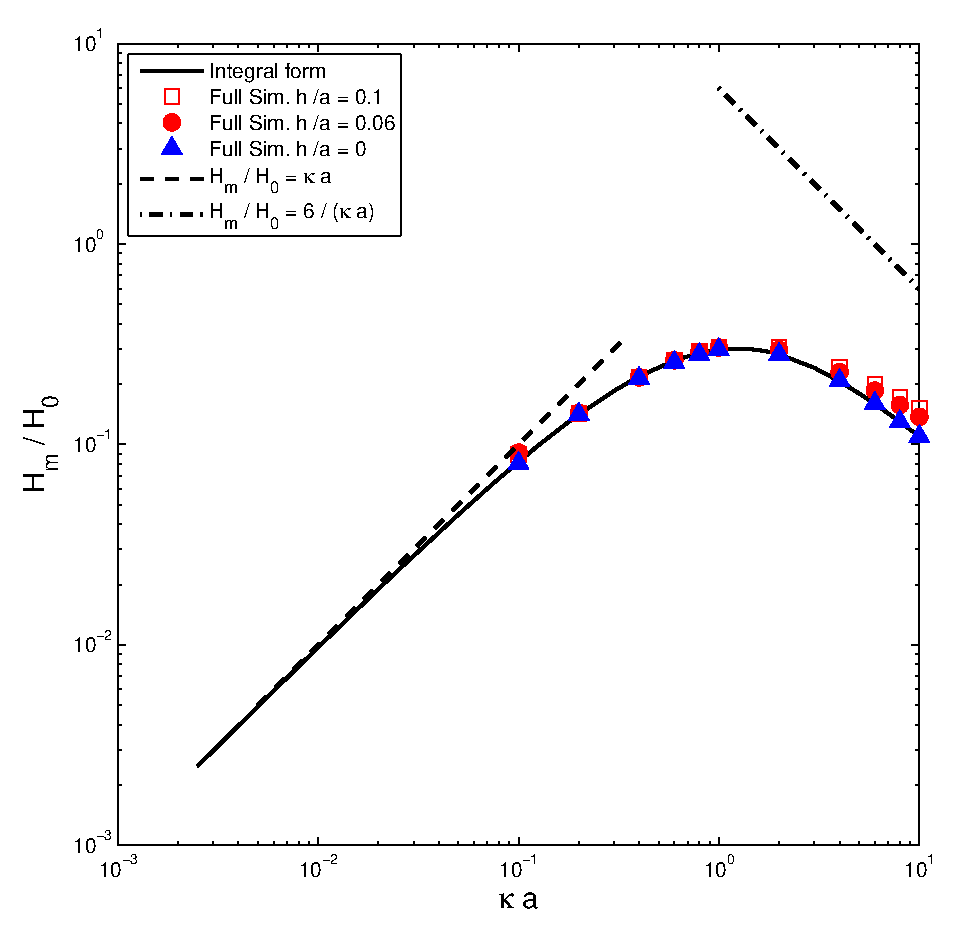
\includegraphics[width=0.50\textwidth]{finite_thickness/HmOverH0LogLog3}
\caption{The electroosmotic coefficient $H_{m}$, scaled by $H_0$ (Equation \ref{H0_defn}), for a membrane of thickness $h=0$, as a function of $a\kappa$. Solid line, analytic result (Equation \ref{reciprocal_integral}); dashed line, asymptote (Equation \ref{H_m_akappa_small}) for $a\kappa\ll 1$;
triangles: full PNP numerical computation ($h=0$). The dot-dashed line shows $H_{m}/H_0=6/(a\kappa)$ with the expected slope for large $a\kappa$. Squares and circles show electroosmotic coefficients $H/H_0$ for non-zero membrane thickness $h>0$, computed by numerical integration of the full PNP equations: solid circles  $h/a=0.06$; open squares $h/a=0.1$.}
\label{Fig:H_m_log_log}
\end{figure}

The membrane has zero thickness, so that there is always a region near
the edge of the pore where the Debye length $\kappa^{-1}$ cannot be
considered small compared with $h$:
Smoluchowski's analysis for thin charge
clouds, which would predict $H=6H_0/(a\kappa)$ if $\zeta_m$ took the
uniform value $(\epsilon\kappa)^{-1}\sigma_m$,
therefore cannot automatically be invoked when $a\kappa\gg 1$.
However, if we set up a local coordinate $s$ indicating distance from
the edge of the pore, both the electric potential $\chi$ (Equation \ref{chi_m})
and the fluid velocity $\mathbf{G}^m$ (Equation \ref{u_membrane})
vary as $s^{1/2}$ when $s\ll a$ (i.e. near the pore edge).
The charge cloud density $\rho_0$ decays over a lengthscale $\kappa^{-1}$,
and only counter-ions of membrane surface charge within a distance $\kappa^{-1}$
from the edge contribute to $\rho_0$ within the hole. The contribution
of the edge to the integral (Equation \ref{reciprocal_integral})
is therefore $O((a\kappa)^{-1})$,
as was similarly found for the electrophoretic velocity of a charged disk \cite{Sherwood1995}.
We therefore expect
$H_m\sim H_0/(a\kappa)$ when $a\kappa\gg 1$. The data in
Figure \ref{Fig:H_m_log_log} do not extend to sufficiently high
values of $a\kappa$ to allow us to estimate the asymptote with
any accuracy, and for the figure we simply indicate the line
$H_m/H_0=6/(a\kappa)$ suggested by the Smoluchowski analysis.
A similar reduction in the broadside electrophoretic velocity of a disk
below the value predicted by Smoluchowski was
noted by Sherwood \& Stone. \cite{Sherwood1995}
Individual points in Figure \ref{Fig:H_m_log_log}
indicate results obtained from full numerical solutions of
the Poisson-Nernst-Planck equations in a symmetric electrolyte
at low applied potential and low surface charge. 
In the computations, the length of
the reservoirs in the $z$ direction was equal to their
radius $b$, with $b=\max(10a,10\kappa^{-1})$.
Other details of the computations are reported in section \ref{sec:finite_numerical}.

\subsection{Composite electroosmotic coefficient $H_{\rm comp}$}
\label{subsec:finite_composite2}
When $h>0$ it is natural to suppose that the electric field
outside
the membrane pumps fluid towards the cylindrical pore at a rate
\begin{equation}
Q_{me}\approx H_m(\phi_1-\phi_2),
\label{q_me}
\end{equation}
and the electric field within the cylindrical pore
pumps fluid through the pore at a rate
\begin{equation}
Q_{ce}\approx H_c\phi_2.
\label{q_ce}
\end{equation}
However, in general, $Q_{me}$ (Equation \ref{q_me}) and
$Q_{ce}$ (Equation \ref{q_ce}) differ, and a pressure $\pm p_2/2$ builds
up at $z=\pm h/2$ (i.e. at the entrance and exit to the cylindrical pore)
in order to ensure that the volumetric flow rate is
continuous. We now determine this pressure $p_2$.

Consider a membrane of zero thickness ($h=0$), with pressure $p=p_1/2$
(above the reference ambient pressure)
at infinity on the side $z>0$, and with $p=-p_1/2$ at infinity on
the other side. The pressure within the hole in the membrane is
\begin{equation}
p=0,\quad z=0,\ r<a,\ h=0.
\end{equation}
The fluid velocity generated by the pressure difference $p_1$
across the membrane is
$\mathbf{u}=p_1\mathbf{G}^m$ (Equation \ref{u_membrane}),
and the corresponding volumetric flow rate is \cite{Happel&Brenner} %% revision - a cite added for flow rate 
\begin{equation}
Q_{mh}=G_mp_1,\quad G_m=-\frac{a^3}{3\mu}.
\end{equation}

If $h>0$ we approximate the pressure field in the fluid in much the same way as
we approximated the electrical potential within the fluid:
we patch a linearly varying pressure $p(z)$ within the
cylindrical pore to the pressure field outside a membrane of zero thickness,
and we take the pressure over the two ends $z=\pm h/2$ of the cylindrical
pore to be $\pm p_2/2$.
Thus the pressure within the pore is approximated as
\begin{equation}
p=\frac{p_2}{h}z,\quad r<a,\ |z|<h/2,
\end{equation}
the fluid velocity within the pore is
\begin{equation}
\mathbf{u}=p_2\mathbf{G}^c,
\label{u_c}
\end{equation}
and the volumetric flow rate within the pore is
\begin{equation}
Q_{ch}=G_cp_2,\quad G_c=-\frac{\pi a^4}{8h\mu}.
\label{G_c}
\end{equation}
Outside the cylindrical pore, the fluid velocity is assumed now to be
\begin{equation}
\mathbf{u}=(p_1-p_2)\mathbf{G}^m(r,z-h/2),\quad z>h/2,
\label{u_m}
\end{equation}
with $u_r(r,z)=-u_r(r,-z)$ and $u_z(r,z)=u_z(r,-z)$. 
The volumetric flow rate outside the membrane is now
\begin{equation}
Q_{mh}=G_m(p_1-p_2),\quad G_m=-\frac{a^3}{3\mu}.
\label{G_m}
\end{equation}
We have
ensured that the pressure (but not the fluid
velocity nor the volumetric flow rate) is continuous across the ends
$z=\pm h/2$ of
the cylindrical pore.

When an electric field generates an electroosmotic velocity, the
volumetric flow rates within the cylindrical pore and outside the
membrane are identical if $p_2$ is such that $Q_{mh}+Q_{me}=Q_{ch}+Q_{ce}$,
i.e. if
\begin{equation}
G_m(p_1-p_2)+H_m(\phi_1-\phi_2)=G_cp_2+H_c\phi_2.
\end{equation}
But the pressure at infinity is zero in the electroosmotic problem, so
$p_1=0$, and $\phi_2$ is given by Equation \ref{phi_2}.
Hence
\begin{equation}
p_2=
\frac{H_mR_m-H_cR_c}{(G_m+G_c)(R_m+R_c)}\phi_1,
\end{equation}
and the total electro-osmotic flow is
\begin{equation}
Q_E=Q_{me}+Q_{mh}=
\frac{(G_mR_cH_c+G_cH_mR_m)}{(R_m+R_c)(G_m+G_c)}\phi_1=H_\text{comp}\phi_1.
\label{flow_rate_lumped_parameter}
\end{equation}
An alternative derivation of this approximate composite
$H_\text{comp}$ (Equation \ref{flow_rate_lumped_parameter}) is given in the next
section.

Inserting into Equation \ref{flow_rate_lumped_parameter}
the various estimates for $G_m$ (Equation \ref{G_m}), $G_c$ (Equation \ref{G_c}),
$R_m$ (Equation \ref{Im_h0}) and $R_c$ (Equation \ref{I_c}),
we obtain
\begin{equation}
H_\text{comp}=
\frac{\left(H_m+\frac{16 h^2}{3\pi^2a^2}H_c\right)}
{\left(1+\frac{2h}{\pi a}\right)
\left(1+\frac{8h}{3\pi a}\right)}.
\label{H_comp}
\end{equation}
For small $h/a$ the approximate composite $H_\text{comp}$
is
larger than $H_m$ if
\begin{equation}
\frac{H_c}{H_m}>\frac{7\pi a}{8h}.
\label{H_c_for_H_comp_increasing}
\end{equation}
%%%%%% revision -- referee 2 %%%%
Experimental arrangements sometimes involve measurements at fixed current,
and a coefficient $K_\text{comp}$ that gives the electroosmotic
flux per unit current is therefore useful.
This quantity may be obtained readily from Equation \ref{I_c}, Equation \ref{phi_2} and Equation \ref{flow_rate_lumped_parameter}:
\begin{equation} 
K_\text{comp} = - \frac{Q_E}{I_c} = 
\frac{(G_mK_c+G_cK_m)}{(G_m+G_c)} = 
\frac{\left(K_m+\frac{8h}{3\pi a}K_c\right)}
{\left(1+\frac{8h}{3\pi a}\right)},
\label{K_comp}
\end{equation}
which changes from $K_m$ when $h=0$ to $K_c$ when $h\gg a$.

\subsection{Composite electroosmotic coefficient $H_{\rm comp}$
derived via the reciprocal theorem}
\label{subsec:finite_composite1}
We now show that approximations to the electric potential $\chi$ and
pressure-driven velocity $\mathbf{G}$ within a pore of non-zero length $h>0$,
when inserted into the integral expression (Equation \ref{reciprocal_integral})
for the electroosmotic
volume flux, lead to an approximate electroosmotic coefficient
identical to $H_\text{comp}$ (Equation \ref{H_comp}) obtained in the previous section.

We have already shown that we may approximate the electric potential
by a composite potential (Equation \ref{approx_chi_c}), (Equation \ref{approx_chi_m}), of the form
\begin{subeqnarray}
\chi&=&\left(\frac{z}{h}\right)\frac{R_c\phi_1}{R_m+R_c},\hskip 80pt |z|<h/2,
\\
&=&\frac{R_c\phi_1}{2(R_m+R_c)}+\frac{R_m\phi_1}{R_m+R_c}
\tilde\chi_m(r,z-h/2),
\hskip 10pt z>h/2,
\\
&=&\chi(r,-z),\hskip 90pt z<0.
\label{chi_approx_composite}
\end{subeqnarray}
%%% JOHN: I modified this sentence because here you are talking about 
% the flow generated under the sole influence of pressure. I worried that 
% this point would be lost on the reader OK, noted.
%We now create a similar approximation for the fluid velocity.
We now create a similar approximation for the fluid velocity for flow 
through a membrane of thickness $h$ subjected only to a pressure drop $p_1$ 
but no applied potential drop.
%%%%%%%%%%%
We suppose that in $z>h/2$ the fluid velocity is given by (Equation \ref{u_m}),
corresponding to flow outside a membrane of zero thickness, and that
within the cylindrical pore the fluid velocity is given by
(Equation \ref{u_c}). Continuity of the volumetric flow rates (Equation \ref{G_c}), (Equation \ref{G_m}) at the entrance to
the cylindrical pore requires that the pressure
$\pm p_2/2$ at the two ends of the pore satisfies
\begin{equation}
G_cp_2=G_m(p_1-p_2),
\end{equation}
so that
\begin{equation}
p_2=\frac{G_mp_1}{G_c+G_m}.
\end{equation}
Hence our approximation to the fluid velocity
is $\mathbf{u}=\mathbf{G}p_1$, with
\begin{subeqnarray}
\mathbf{G}&=&
\frac{G_m}{G_c+G_m}\mathbf{G}^c(r,z),\hskip 65pt |z|<h/2,
\\
&=&\frac{G_c}{G_c+G_m}\mathbf{G}^m(r,z-h/2),\hskip 30pt z>h/2.
\label{G_approx_composite}
\end{subeqnarray}
The (small) errors involved in this approximation are discussed by
Dagan et al. \cite{dagan1982}.

We now use the approximations (Equation \ref{chi_approx_composite}) and
(Equation \ref{G_approx_composite}) in the integral (Equation \ref{reciprocal_integral}) in order to
compute the electroosmotic volumetric flow rate. But the integration
splits naturally into an integral over the cylindrical pore and an
integral over the regions outside the membrane. The integral over the
cylindrical pore is exactly the integral required to determine
the electroosmotic flow rate $H_c$ (Equation \ref{Hc_defn}) in a cylinder, and the
integral outside the membrane is exactly that required to determine
$H_m$ (Equation \ref{Hm_defn}). Hence the integral yields the composite
electroosmotic flow rate
\begin{equation}
H_\text{comp}= \frac{G_cR_mH_m}{(G_c+G_m)(R_m+R_c)}
+\frac{G_mR_cH_c}{(G_c+G_m)(R_m+R_c)}
=\frac{G_cR_mH_m+G_mR_cH_c}{(G_c+G_m)(R_m+R_c)},
\end{equation}
identical to (Equation \ref{flow_rate_lumped_parameter}), obtained in section \ref{subsec:finite_composite2} by
elementary methods.

\subsection{Predictions of the composite electroosmotic coefficient}
\begin{figure}[ht]
\includegraphics[width=\textwidth]{finite_thickness/finite_pore_pic3.eps}
\caption{\label{Fig:H_comp}
The electroosmotic coefficient $H$ scaled by $H_0$ (Equation \ref{H0_defn}) for
$\sigma_m=\sigma_c$, as a function of $h/a$, for
(a) $a\kappa=10$, (b) $a\kappa=2$, (c) $a\kappa=1$,
 (d) $a\kappa=0.1$.
Solid lines, $H_{comp}$ (Equation \ref{H_comp});
solid circles: full PNP numerical computation.}
\end{figure}

\begin{figure}[ht]
\includegraphics[width=\textwidth]{finite_thickness/finite_pore_pic7.eps}
\caption{The results of Figure \ref{Fig:H_comp}, presented in terms of the electroosmotic coefficient $K=HR_{tot}$ scaled by $K_0$ (Equation \ref{K0_defn}) for $\sigma_m=\sigma_c$, as a function of $h/a$, for (a) $a\kappa=10$, (b) $a\kappa=2$, (c) $a\kappa=1$, (d) $a\kappa=0.1$. Solid lines, $K_{comp}$ (Equation \ref{K_comp}); solid circles: full PNP numerical computation.}
\label{Fig:K_comp}
\end{figure}

Figure \ref{Fig:H_comp} shows $H_\text{comp}$ (Equation \ref{H_comp}) as a function of $h/a$, for four
different values of $a\kappa$, with $\sigma_m=\sigma_c$. Also shown are the results of full numerical
computations based on the
Poisson-Nernst-Planck equations \cite{mao2014}
and described in section \ref{sec:finite_numerical}. 
The coefficient $H_c$ (Equation \ref{Hc_defn})
is proportional to $h^{-1}$ and is very large when the
pore length $h$ is small, leading to a large electroosmotic coefficient
$H_\text{comp}$. The action of the electric field
acting on charge confined within the cylindrical pore
is much more efficient at creating fluid motion than is the
weaker electric field acting on charge outside the pore.
We see that for $a\kappa\ge 1$ the
approximate analysis captures the main features of the full numerical
results, and it is clear from (Equation \ref{H_comp}) that it also has the
correct limits as $h/a\rightarrow 0$ and
$h/a\rightarrow\infty$. However,
it is also evident from Figure \ref{Fig:H_comp}(d)
that the theory is unsatisfactory when
$a\kappa\ll 1$.

The results of Figure \ref{Fig:H_comp}
are presented in terms of the coefficient $K_\text{comp}$
(Equation \ref{K_comp}) in Figure \ref{Fig:K_comp}. Both $K_\text{comp}$
and the full numerical results now increase monotonically with $h$,
with a final end point $K_\text{comp}=K_c$ that is independent of
$h$ when $h\gg a$. Figure \ref{Fig:K_comp}, like Figure \ref{Fig:H_comp},
shows that the theory leading to $K_\text{comp}$ is
inadequate when $a\kappa\ll 1$.
We discuss this limit in section \ref{sec:finite_overspill}, where
we shall show that when $a\kappa\ll 1$ some of the charge cloud of ions
that neutralizes the surface charge on the cylindrical wall of the pore
spills out of the ends of the pore, where it is less effective at generating
electroosmotic flow. The scenario is shown schematically in 
Figure \ref{Fig:schematic_overspill}.

\section{Numerical simulation}
\label{sec:finite_numerical}
The time-independent PNP--Stokes equations governing the electrical potential
$\phi$, the ionic number density of the $i$th ionic species $n^i$
($i=1,\dots,N$), the fluid velocity $\mathbf{u}$ and fluid pressure $p$
are
\begin{eqnarray}
\epsilon \nabla^2 \phi + \sum_{i=1}^{N} z_i e n^i & = & 0,
\label{eq:poisson_finite}
\\
\nabla\cdot\left\lbrack n^i\mathbf{u} -\omega^i(kT \nabla
n^i + ez_in^i\nabla\phi) \right\rbrack&=&0 ,
\label{eq:NP}
\\ 
-\nabla p + \mu \nabla^2 \mathbf{u} -  \nabla \phi \sum_{i=1}^{N} z_ien^i & = & 0, \label{eq:stokes_finite}\\
\nabla \cdot \mathbf{u} & = & 0, \label{eq:continuity_finite}
\end{eqnarray}
where $z_i$ is the valence of the $i$th ionic species and $\omega^i$
its mobility. Here we restrict our attention to the case
$N=2$, with $z_1=-z_2=1$.

We used a finite volume numerical scheme to
solve the system of coupled equations (Equation \ref{eq:poisson_finite})-(Equation \ref{eq:continuity_finite}) 
in the axisymmetric geometry depicted in Figure \ref{Fig:schematic}.
Thus, we considered a cylindrical pore of radius $a$ and length $h$ connecting two large cylindrical reservoirs of radius $b$. The lengths of AB and EF in our simulation were also taken to be $b$, which was kept much larger than either $a$ or the Debye length 
$\kappa^{-1}$ so that the reservoirs were effectively infinite.

{\it Boundary conditions.} At A and F, the two ends of the reservoirs, ion concentrations were set equal to the concentration in the bulk electrolyte (i.e. $n^i = n^{i}_{\infty}$); a potential difference $\Delta V$ was applied across the system by setting $\phi$ to $\pm \Delta V/2$ respectively at A and F where the pressures were set equal to the bulk pressure, $p = p_\infty$. At AB and EF, the side walls of the cylindrical reservoir, the radial component of the electric field, ionic flux and velocity were all set to zero, as was the tangential shear stress, in order to minimize the effect of these boundaries.
The last condition was imposed as the cylindrical reservoirs merely represent a convenient 
computational domain; the walls of the real physical reservoir are far enough away from the pore to be essentially irrelevant.
At the membrane and pore surfaces BC, CD and DE, a no--flux condition was used for (Equation \ref{eq:NP}), and a no--slip condition was used for the flow. At solid-fluid interfaces (with unit normal $\hat{n}$)
the electric potential is continuous but the normal component of the electric field undergoes a jump, with
$[ \epsilon \mathbf{E}\cdot \hat{n} ] = \sigma_m$ at BC and DE, 
and $[ \epsilon \mathbf{E}\cdot \hat{n} ] = \sigma_c$ at CD.

An electrohydrodynamic solver was implemented to solve the system described above using the OpenFOAM CFD library \cite{OPENFOAM}, a C++ library designed for computational mechanics. A structured mesh was constructed by means of the polyMesh
meshing tool within OpenFOAM. The grid was refined near the membrane and pore surfaces to resolve the Debye layer. Grid independence was checked in all cases by refining the grid and verifying that the 
solution did not change within specified tolerances.

For the finite volume discretization of the governing equations, central differences were used for all diffusive terms in (Equation \ref{eq:NP}) and viscous terms in (Equation \ref{eq:stokes_finite}). A second--order upwind scheme was used for the convective terms in (Equation \ref{eq:NP}). The discretized linear system was solved using a pre-conditioned conjugate gradient solver if the matrix was symmetric or a pre-conditioned bi--conjugate gradient solver if the matrix was 
asymmetric \cite{ferziger&peric}. 

An iterative scheme was used to solve the PNP--Stokes equations. Initially, the flow velocity 
was set to zero. Equations  (Equation \ref{eq:poisson_finite}) and (Equation \ref{eq:NP}) were then solved sequentially in a loop with under-relaxation (to ensure stability of the nonlinear PNP system) until the absolute residual was smaller than a specified tolerance -- in our case, $10^{-6}$.
 The electric force density $- \nabla \phi\sum_i z_ien^i $ was then obtained from this solution and used 
 as an explicit external forcing in the solution of the incompressible Stokes flow problem,
 (Equation \ref{eq:stokes_finite}) and (Equation \ref{eq:continuity_finite}), solved by means of the SIMPLE algorithm.  The flow field so computed was then substituted into (Equation \ref{eq:NP}) and the PNP equations were solved again using the updated flow field. An outer loop was constructed to iterate over the PNP loop and Stokes flow module, until the solution changed negligibly between two outer iterations.

Our main object of interest is the volumetric flux, $Q$. This was obtained by numerically integrating the axial velocity over the plane $z = 0$.
At the low voltages employed, the linear relation found between 
$Q$ and $\Delta V$ leads to the electroosmotic coefficient $H = Q/ \Delta V$,
shown as discrete points in Figures \ref{Fig:H_m_log_log}, \ref{Fig:H_comp},
\ref{Fig:K_comp}
and \ref{Fig:H_comp_akappa_small}.
The amount of charge within the pore was determined by numerical integration,
and used to obtain the quantities $h_\text{lost}$ and $h_\text{gained}$
reported below in Table 1.


\section{Charge overspill from the ends of the pore, $a\kappa\ll 1$\label{sec:finite_overspill}}
\subsection{Overspill of charge from the end of a semi-infinite pore}
\begin{figure}[ht]
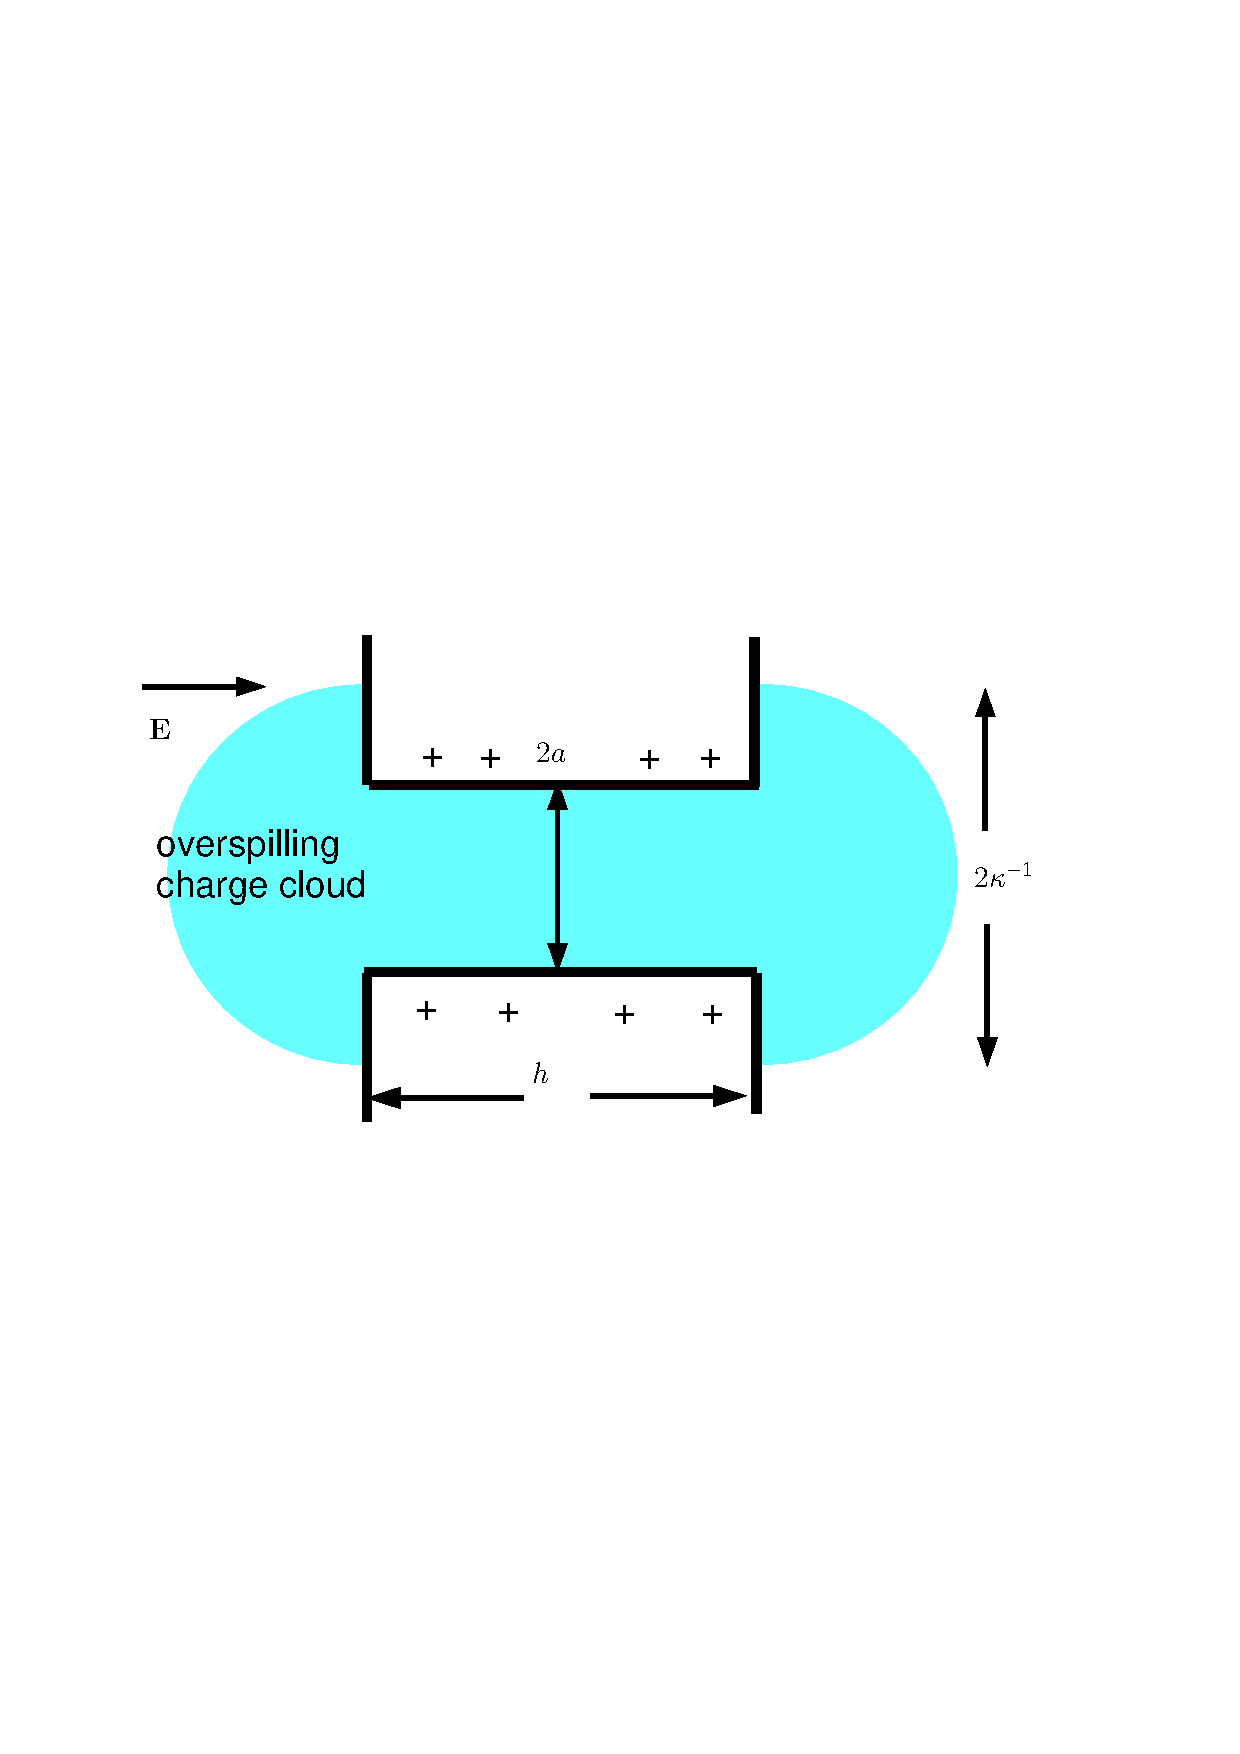
\includegraphics[width=0.6\textwidth]{finite_thickness/finite_pore_pic5}
\caption{When the Debye length $\kappa^{-1}$ is large compared with the pore radius $a$, the cloud of counter ions associated with the charged cylindrical wall of the pore spills out of the ends of the pore.}
\label{Fig:schematic_overspill}
\end{figure}

We consider a cylindrical pore of radius $a$, with surface charge density
$\sigma_c$. When the Debye length $\kappa^{-1}\gg a$,  the
equilibrium potential $\phi_0$ (Equation \ref{phi0_cylinder}) in an infinitely long cylinder can be expanded as
\begin{equation}
\phi_0=\phi_a
\left(1+\frac{(\kappa   r)^2}{4}+\cdots\right),
\end{equation}
where
\begin{equation}
\phi_a=\frac{\sigma_c}{\epsilon\kappa I_1(\kappa a)}
\approx\frac{2\sigma_c}{\epsilon\kappa(\kappa a)}.
\label{phi1_defn}
\end{equation}
Thus the equilibrium potential $\phi_0$ and charge density
$\rho_0=-\epsilon\kappa^2\phi_0$
within the charge cloud vary little over the
cross-section of the pore. On the other hand, if the cylinder is not
infinitely long and uniform, $\phi_0$ and $\rho_0$ vary
in the axial ($z$) direction with a length scale $\kappa^{-1}$.
We can therefore consider the equilibrium potential $\phi_0$ 
within the cylindrical pore to be a function only of
$z$ \cite{singer2009}.



We first consider a semi-infinite, charged cylindrical pore going from $z=0$
to $z=\infty$. The equilibrium potential $\phi_0$
satisfies a one-dimensional Poisson-Boltzmann
equation,
\begin{equation}
\frac{\text{d}^2\phi_0}{\text{d}z^2}=-\kappa^2\phi_0.
\label{1D_PB_eqn}
\end{equation}
The solution that tends to the uniform potential $\phi_a$ within the
pore as $z\rightarrow\infty$ far from the pore end at $z=0$, is
\begin{equation}
\phi_0=\phi_a-A\exp(-\kappa z),
\label{phi_semi_infinite}
\end{equation}
for some unknown constant $A$. 
The charge density within the charge cloud
inside the pore is $-\epsilon\kappa^2\phi_0$, and when the cylindrical
pore is infinite (and hence uniform) the charge per unit length in the
charge cloud is $-\pi a^2\epsilon\kappa^2\phi_a=-2\pi\sigma_ca$, equal
and opposite to the charge per unit length on the pore walls. When the
pore is semi-infinite, with a non-uniform charge
cloud (Equation \ref{phi_semi_infinite}), the
total charge that is lost from within the pore is
\begin{equation}
q_\text{lost}=-\pi a^2\epsilon\kappa^2\int_0^\infty (\phi_a-\phi_0)\,\text{d}z
=-\pi a^2\kappa\epsilon A.
\label{q_lost_one_end}
\end{equation}
At the end of the pore ($z=0$) the potential
is $\phi=\phi_a-A$.  

In $z<0$ the charge
cloud is no longer confined by the walls of the cylindrical pore
and spreads out radially: it is no longer possible to assume that
$\phi_0$ is a function of $z$ alone. 
We therefore need to solve the linearized Poisson-Boltzmann equation in the half-space $z<0$,
with $\phi_0=\phi_a-A$ over the region $z=0$, $r<a$ and
$\partial\phi_0/\partial z=0$ on $z=0$, $r>a$. At large distances from the
end of the pore, the potential decays as $\exp(-\kappa R)/R$,
where $R=(z^2+r^2)^{1/2}$ is a spherical polar coordinate,
but in the important region $R=O(a)$ the potential can be approximated by
the electrostatic potential corresponding to a solution of the Laplace
equation (i.e. $\kappa=0$). Hence, from (Equation \ref{chi_m}),
\begin{equation}
\phi_0=(\phi_a-A)\frac{2}{\pi}\tan^{-1}\left(\frac{1}{\sinh\xi}\right).
\label{laplace_disk}
\end{equation}
To relate the potential (Equation \ref{laplace_disk}) to the amount of charge
in the overspilling charge cloud (in $z<0$), we note that
the charge on one side of a charged disk at uniform potential
$(\phi_a-A)$ in unbounded space is 
$q=4a\epsilon(\phi_a-A)$.
Alternatively, one can argue that
far from the plane $z=0$, the spherical distance $R\approx a\cosh\xi$,
so that the potential (Equation \ref{laplace_disk}) is approximately
\begin{equation}
\phi_0\approx (\phi_a-A)\frac{2a}{\pi R}.
\end{equation}
In a spherically symmetric geometry this field corresponds to the far
field around a point charge of magnitude $8a\epsilon(\phi_a-A)$,
and the total surface charge on one side of the disk is 
$q=4a\epsilon(\phi_a-A)$, in agreement with the charge obtained by considering
the capacitance of the disk. The charge in the overspill charge cloud in $z<0$
is equal and opposite to $q$, and is therefore
\begin{equation}
q_\text{overspill}=-4a\epsilon\phi_0(z=0)=-4a\epsilon(\phi_a-A).
\label{capacitance_disk}
\end{equation}
But the total charge (Equation \ref{capacitance_disk}) in the overspill
outside the end of the pore must be
equal to the charge (Equation \ref{q_lost_one_end})
that has been lost from within the pore.
Hence
\begin{equation}
4a\epsilon(\phi_a-A)=\pi a^2\kappa\epsilon A,
\end{equation}
so that
\begin{equation}
A=\frac{\phi_a}{1+\pi a\kappa/4},
\end{equation}
and the potential at the end of the pore is
\begin{equation}
\phi_a-A=\frac{\phi_a}{1+4/(\pi a\kappa)}.
\end{equation}
The charge that has been lost from the end of the
pore is equivalent to the charge usually found in a pore of length
\begin{equation}
h_\text{lost}=-\frac{q_\text{overspill}}{2\pi a\sigma_c}
=\frac{4}{4\kappa+\pi a\kappa^2}.
\label{h_lost_one_end}
\end{equation}
The loss of charge implies that the combined charge cloud and wall
surface charge
over a cross section of constant $z$ are no longer electrically neutral,
as pointed out by Baldessari and Santiago \cite{baldessari2008a, baldessari2009a}.

\subsection{Overspill from the two ends of a finite pore}
We can now perform the same analysis for a pore that
occupies the region $-h/2<z<h/2$. The equilibrium
potential within the pore has the form
\begin{equation}
\phi_0=C-B\cosh(\kappa z),
\label{phi0_inside_two_ends}
\end{equation}
where we have chosen the solution that is symmetric about the centre of
the pore at $z=0$. The charge that has been lost from within the
pore is
\begin{equation}
q_\text{lost}=-\epsilon\kappa^2\pi a^2
\left(\int_{-h/2}^{h/2}(\phi_0-\phi_a)\,\text{d}z\right)
=\epsilon\pi a^2\kappa^2\left\lbrack
\frac{2B}{\kappa}\sinh\left(\frac{\kappa h}{2}\right)+(\phi_a-C)h\right\rbrack.
\label{q_lost_inside_two_ends}
\end{equation}
The total flux of electric field through the two ends of the pore
is
\begin{equation}
2\pi a^2\left.\frac{\partial\phi_0}{\partial z}\right|_{z=h/2}
=-2\pi a^2\kappa B\sinh\left(\frac{\kappa h}{2}\right).
\label{flux_though_two_ends}
\end{equation}
Comparing (Equation \ref{q_lost_inside_two_ends}) and
(Equation \ref{flux_though_two_ends}) we conclude that $C=\phi_a$. The potential
over the ends of the pore is
\begin{equation}
\phi_0(h/2)=\phi_0(-h/2)=\phi_a-B\cosh(\kappa h/2).
\end{equation}
The total charge in the two overspill charge clouds is therefore,
by (Equation \ref{capacitance_disk}),
\begin{equation}
q_\text{overspill}=-8a\epsilon\left\lbrack\phi_a
-B\cosh\left(\frac{\kappa h}{2}\right)\right\rbrack,
\label{q_overspill_two_ends}
\end{equation}
and this must be equal to the charge (Equation \ref{q_lost_inside_two_ends})
lost from within the pore. Hence
\begin{equation}
B=\frac{4\phi_a}{4\cosh(\kappa h/2)+\pi a\kappa\sinh(\kappa h/2)}
\label{B}
\end{equation}
and
\begin{equation}
\phi_a-B\cosh\left(\frac{\kappa h}{2}\right)=
\frac{\phi_a\pi a\kappa\sinh(\kappa h/2)}{4\cosh(\kappa h/2)+\pi
  a\kappa\sinh(\kappa h/2)}.
\label{phi_a_minus_B_cosh}
\end{equation}
The total charge that has been lost (from the two ends) is equivalent to a
total lost length
\begin{eqnarray}
h_\text{lost}=-\frac{q_\text{overspill}}{2\pi a\sigma_c}&=&
\frac{8\sinh(\kappa h/2)}
{4\kappa\cosh(\kappa h/2)+\pi a\kappa^2\sinh(\kappa h/2)}
\label{h_lost_two_ends}
\\
&\sim&\frac{8}{4\kappa+\pi a\kappa^2},\hskip 30pt \kappa h\gg 1,
\label{h_lost_two_ends_h_large}
\\
&\sim&\frac{4h}{4+\pi ah\kappa^2/2}
,\hskip 30pt \kappa h\ll 1.
\label{h_lost_two_ends_h_small}
\end{eqnarray}
We see from eqs (Equation \ref{h_lost_one_end}) and (Equation \ref{h_lost_two_ends_h_large}) 
that when $\kappa h\gg 1$ the lost charge is twice that lost
from a single end of a pore. We also note that $h-h_\text{lost}>0$, and that
when the pore is short ($\kappa h\ll 1$) the amount of charge
remaining within the cloud within the pore is proportional to
\begin{equation}
h-h_\text{lost}
\sim\frac{\pi a \kappa^2h^2}{8+\pi ah\kappa^2}
,\hskip 30pt \kappa h\ll 1.
\label{h_min_h_lost_h_small}
\end{equation}

\subsection{Overspill from the membrane surface into the pore}
\label{subsec:finite_overspill4-3}
If the cylindrical
pore itself is uncharged, but the membrane surfaces are charged, ions
from the charge cloud adjacent to the membrane surface
are able to move into the ends of the pore.

If the membrane has zero thickness,
the charge density $\rho_0$ in the equilibrium charge cloud is
given by (Equation \ref{eq:rho0_finite}), and
both $\rho_0$ and the potential $\phi_0=-\rho_0/(\epsilon\kappa^2)$
vary over the area of the pore. Nevertheless, we may work out the mean potential
over the circular pore,
\begin{equation}
\overline{\phi}_0=-\frac{1}{\epsilon\kappa^2\pi a^2}
\int_0^a 2\pi r\rho_0\,\text{d}r
=\frac{2\sigma_m}{\epsilon a}
\left\lbrack\frac{a}{2\kappa}-
 \int_0^\infty
\frac{aJ_1(as)J_1(as)}{s(\kappa^2+s^2)^{1/2}}\,\text{d}s
 \right\rbrack,
\end{equation}
where, when $a\kappa\ll 1$,
\begin{equation}
\int_0^\infty
\frac{aJ_1(as)J_1(as)}{s(\kappa^2+s^2)^{1/2}}\,\text{d}s
\approx a^2\int_0^\infty
\frac{J_1(t)J_1(t)}{t^2}\,\text{d}t
=\frac{4a^2}{3\pi}.
\end{equation}
Thus when the membrane has zero thickness (and there is no
cylindrical pore into which ions can escape)
the absence of surface charge over
the area of the pore
changes the average potential over the opening from 
the value
$\phi_0=\sigma_m/(\epsilon\kappa)$ due to a uniformly charged surface
to $\beta\sigma_m/(\epsilon\kappa)$, where
\begin{equation}
\beta\approx 1-\frac{8a\kappa}{3\pi},\hskip 20pt a\kappa \ll 1.
\label{beta_defn}
\end{equation}

We now consider the charge
that leaks into a pore of length $h>0$ from the charge clouds on either
side of the membrane.
We suppose that the potential on the planes
$z=\pm h/2$ is perturbed by an amount $D$, and becomes
\begin{equation}
\phi_0=\frac{\beta\sigma_m}{\epsilon\kappa}+D,\hskip 20pt z=\pm h/2.
\label{underspill_perturbed_potential}
\end{equation}
Within the pore, the potential obeys the 1-dimensional
Poisson-Boltzmann equation (Equation \ref{1D_PB_eqn}), with solution
\begin{equation}
\phi_0=\left(\frac{\beta\sigma_m}{\epsilon\kappa}+D\right)
\frac{\cosh(\kappa z)}{\cosh(\kappa h/2)},
\end{equation}
and the additional charge within the pore is
\begin{equation}
q_\text{in}-\epsilon\kappa^2\pi a^2\int_{-h/2}^{h/2}\phi_0\,\text{d}z
=-\pi a^2\left(\beta\sigma_m+D\epsilon\kappa\right)
\frac{2\sinh(\kappa h/2)}{\cosh(\kappa h/2)}.
\end{equation}
Outside the pore, the perturbed potential
(Equation \ref{underspill_perturbed_potential}) is associated with
a total additional charge (Equation \ref{capacitance_disk})
\begin{equation}
q_\text{out}=-8a\epsilon D
\label{q_out_underspill}
\end{equation}
on the two sides of the membrane.
But the total change in charge caused by this redistribution must be zero,
i.e. $q_\text{in}+q_\text{out}=0$. Hence
\begin{equation}
\pi a^2\left(\beta\sigma_m+D\epsilon\kappa\right)
\frac{2\sinh(\kappa h/2)}{\cosh(\kappa h/2)}
+8a\epsilon D=0,
\end{equation}
i.e.
\begin{equation}
D=-\frac{\pi a\beta\sigma_m\sinh(\kappa h/2)}
{[4\cosh(\kappa h/2)+\pi a\kappa\sinh(\kappa h/2)]\epsilon}.
\end{equation}
The total charge $q_\text{in}=-q_\text{out}$ (Equation \ref{q_out_underspill})
that leaks into the pore at the two ends
corresponds to the charge inside a uniformly charged
cylinder with surface charge density $\sigma_m$,  of length
\begin{eqnarray}
h_\text{gained}=-\frac{8a\epsilon D}{2\pi a\sigma_m}&=&\frac{4 a\beta\sinh(\kappa h/2)}
{4\cosh(\kappa h/2)+\pi a\kappa\sinh(\kappa h/2)}=\frac{a\kappa\beta}{2}h_\text{lost},
\label{h_gained}
\\
&\sim&\frac{a\kappa\beta h}{2},\hskip 20pt \kappa h\ll 1,
\label{h_gained_h_small}
\\
&\sim&\frac{a\beta}{2+\pi a\kappa},\hskip 20pt \kappa h\gg 1.
\end{eqnarray}
Thus $h_\text{gained}$ (Equation \ref{h_gained}) is smaller than
$h_\text{lost}$ (Equation \ref{h_lost_two_ends}) by a factor $a\kappa\beta/2$.
We can compare the
predictions (Equation \ref{h_lost_two_ends})
and (Equation \ref{h_gained}) against results
obtained from full numerical solution of the nonlinear Poisson-Boltzmann
equation with either $\sigma_m=0$ and
$ae\sigma_c/(\epsilon kT)=a\kappa e\zeta_c/(kT)=0.00273$,
or $\sigma_c=0$ and
$ae\sigma_m/(\epsilon kT)=0.00273$:
results for $a\kappa=0.1$ are given in Table 1. We see that there is
excellent agreement between the numerical computations and the analysis
presented above.

\begin{table}
\begin{center}
\begin{tabular}{|c|c @{\hspace{30pt}} |c|c @{\hspace{30pt}} |c|c|}
\hline
$h/a$&$h\kappa$&\multicolumn{2}{c|}{$h_\text{lost}/a$}
&\multicolumn{2}{c|}{$h_\text{gained}/a$}
\\
\hline
&&theory (Equation \ref{h_lost_two_ends})&numerical&theory (Equation \ref{h_gained})&numerical
\\
\hline
10.0&1.0&8.9186&8.9249&0.4081&0.4119
\\
\hline
1.0&0.1&0.9953&0.9954&0.0455&0.0459
\\
\hline
0.1&0.01&0.1000&0.1000&0.0046&0.0046
\\
\hline
\end{tabular}
\end{center}
\caption{The charge lost from the ends of a charged
pore when the membrane charge density $\sigma_m=0$, in terms of an
equivalent pore length $h_\text{lost}$ (Equation \ref{h_lost_two_ends}),
and the charge gained inside an uncharged pore ($\sigma_c=0$)
from the charge cloud adjacent to the charged membrane surfaces,
in terms of an equivalent pore length $h_\text{gained}$ (Equation \ref{h_gained}).
$a\kappa=0.1$.}
\end{table}


\subsection{Composite electroosmotic coefficient}
We first consider how the electroosmotic coefficients $H_c$ and $H_m$
are modified by the overspill of the charge cloud from inside the
cylindrical pore to outside the membrane.
If a uniform electric field of
strength $E=-\phi_1/h$ is applied between the ends of the pore,
the Navier Stokes equations for steady flow yield the axial velocity profile
\begin{equation}
u=\frac{a^2-r^2}{4\mu}\left(\rho_0E-\frac{{\rm d}p}{{\rm d}z}\right)
\end{equation}
so that the volumetric flow rate is
\begin{equation}
Q=\frac{a^4\pi}{8\mu}\left(\rho_0E-\frac{{\rm d}p}{{\rm d}z}\right).
\label{Q_in_uniform_pore}
\end{equation}
But $Q$ is independent of $z$ (by incompressibility), and the pressure $p$
difference between the two ends of the capillary is zero. Hence, integrating
(Equation \ref{Q_in_uniform_pore}) along the length $h$ of the cylindrical pore,
and noting that
the total amount of charge in the charge cloud remaining within
the pore is
$2\pi a\sigma_c(h-h_\text{lost})$, we find
\begin{equation}
Q=\frac{a^4\pi E}{8h\mu}\int_{-h/2}^{h/2}\rho_0\,\text{d}z
=\frac{\pi a^3\sigma_c(h-h_\text{lost})\phi_1}{4h^2\mu}
=H_c\phi_1,
\label{H_c_underspill}
\end{equation}
which may be compared to the result (Equation \ref{H_c_kappa_small})
which ignores overspill.
The charge cloud outside the pore is enhanced by the overspill, and becomes
(in $z>0$)
\begin{equation}
\rho_0
=-\sigma_m\kappa\exp(-\kappa z)
-\frac{2\epsilon\kappa^2}{\pi}\left\lbrack\phi_a-B\cosh(\kappa h/2)\right\rbrack
\tan^{-1}\left(\frac{1}{\sinh\xi}\right),
\end{equation}
with the final term $[\phi_a-B\cosh(\kappa h/2)]$,
corresponding to the overspill charge cloud
(Equation \ref{phi_a_minus_B_cosh}), being
approximately valid in a volume $O(a^3)$ around the pore, but invalid at large
distance $O(\kappa^{-1})$ from the pore, where the exponential decay
of the charge density
is not captured by the solution (Equation \ref{laplace_disk}) of the Laplace equation.
The volumetric flow rate through a pore of zero thickness created by
a potential difference $\phi_1$
is given by the integral (Equation \ref{reciprocal_integral})
and was shown by Mao et al. \cite{mao2014} to be:
\begin{eqnarray}
Q  &=&  \frac{2a^3\phi_1}{\pi\mu}
\int_0^{\frac{\pi}{2}} d\eta \int_0^\infty \rho_0
\frac{\cos^2\eta\sin\eta}{\cosh\xi} d\xi
\nonumber\\
&=&-\frac{a^3\kappa\sigma_m\phi_1}{3\mu}
-\frac{4\epsilon\kappa^2a^3\phi_1}{\pi^2\mu}(\phi_a-B)
\int_0^{\pi/2}\cos^2\eta\sin\eta\text{ d}\eta \int_0^\infty 
\tan^{-1}\left(\frac{1}{\sinh\xi}\right)\frac{\text{d}\xi}{\cosh\xi}
\nonumber\\
&=&-\frac{a^3\kappa\sigma_m}{3\mu}\phi_1
-\frac{4\epsilon a^3\kappa^2}{3\pi^2\mu}\phi_1(\phi_a-B)I_3,
\label{Q_integral_disk}
\end{eqnarray}
where
\begin{equation}
I_3=
\int_0^\infty 
\tan^{-1}\left(\frac{1}{\sinh\xi}\right)\frac{\text{d}\xi}{\cosh\xi}
=\int_0^\infty \tan^{-1}x\ \frac{\text{d}x}{1+x^2}
=\frac{\pi^2}{8}.
\end{equation}
Hence the electroosmotic flow rate $Q=H_m\phi_1$
due to the charge cloud outside the
membrane is modified, and $H_m$ becomes
\begin{equation}
H_m=\frac{a^3\kappa}{3\mu}\left\lbrack
\sigma_m+
\frac{\pi\sinh(\kappa h/2)\sigma_c}
{4\cosh(\kappa h/2)+\pi a\kappa\sinh(\kappa h/2)}
\right\rbrack.
\label{H_m_overspill}
\end{equation}

If $\sigma_m$ is comparable to $\sigma_c$, then we saw in Section \ref{subsec:finite_overspill4-3} that
the change in the charge within the pore due to the charge cloud outside
the membrane entering the pore is $O(a\kappa)$ smaller than the loss of
charge from the charge cloud within the pore to the regions
outside the membrane. However, this contribution can be included
with very little effort, and becomes important in the limit
$h\rightarrow 0$, when the gain (Equation \ref{h_gained_h_small})
in charge within the pore
from the outside surface charge density $\sigma_m$
is proportional to $h_\text{gained}\propto h$,
whereas the charge cloud (due to $\sigma_c$ within the pore)
remaining within the pore, is
proportional to $h-h_\text{lost}\propto h^2$, by
(Equation \ref{h_min_h_lost_h_small}).
The electroosmotic coefficient $H_c$
for the cylindrical pore (Equation \ref{H_c_underspill}) becomes
\begin{equation}
H_c=\frac{\pi a^3\sigma_c(h-h_\text{lost}+h_\text{gained}\sigma_m/\sigma_c)}
{4h^2\mu},
\label{H_c_overspill_underspill}
\end{equation}
and the electroosmotic coefficient $H_m$ for the charge cloud
outside the membrane (Equation \ref{H_m_overspill}) becomes
\begin{equation}
H_m=\frac{a^3\kappa}{3\mu}\left\lbrack
\sigma_m+
\frac{\pi\sinh(\kappa h/2)(\sigma_c-a\kappa\beta\sigma_m/2)}
{4\cosh(\kappa h/2)+\pi a\kappa\sinh(\kappa h/2)}
\right\rbrack.
\label{H_m_overspill_underspill}
\end{equation}

Now that $H_c$ (Equation \ref{H_c_overspill_underspill}) and 
$H_m$ (Equation \ref{H_m_overspill_underspill})
have been corrected for the effects of overspill
in the two directions, they can be inserted into the expression
(Equation \ref{H_comp})
for the composite electroosmotic coefficient $H_\text{comp}$.
Results are shown in Figure \ref{Fig:H_comp_akappa_small}(a), together
with full numerical solutions of the Poisson-Nernst-Planck equations.
We see that the agreement between theory and computation is much better
than  when overspill is ignored (Figure \ref{Fig:H_comp}(d)). 
Charge overspill or underspill causes the total charge of mobile ions
within the pore to differ
from what might be expected on the basis of net 
electroneutrality of the pore. 
Thus, the driving force is modified leading to deviations from the calculated 
result that ignores such effects. The ``lost length'' $h_\text{lost}$ in (Equation \ref{H_c_overspill_underspill})
restores this effect.
Figure \ref{Fig:H_comp_akappa_small}(b) shows the results of
Figure \ref{Fig:H_comp_akappa_small}(a) expressed in terms of
$K$, rather than $H$, and there is again good agreement between the
theoretical $K_\text{comp}$ and full numerical results.

\begin{figure}[ht]
\includegraphics[width=0.99\textwidth]{finite_thickness/finite_pore_pic8.eps}
\caption{\label{Fig:H_comp_akappa_small}
(a) The electroosmotic coefficient $H$ scaled by $H_0$ (Equation \ref{H0_defn}) for $\sigma_m=\sigma_c$, as a function of $h/a$, for $a\kappa=0.1$, including the effect of overspilling charge clouds. Solid lines $H_\text{comp}$ (Equation \ref{H_comp}), using $H_c$ given by (Equation \ref{H_c_overspill_underspill}) and $H_m$ given by (Equation \ref{H_m_overspill_underspill}); solid circles: full PNP numerical computation. c.f. Fig. \ref{Fig:H_comp}(d), in which overspill was neglected. (b) The same results, presented in terms of $K=R_\text{tot}H$ scaled by $K_0$ (Equation \ref{K0_defn}). Solid lines $K_\text{comp}$ (Equation \ref{K_comp}), using $K_c=R_cH_c$ and $K_m=R_mH_m$; solid circles: full computation. c.f. Fig. \ref{Fig:K_comp}(d).}
\end{figure}

Note that when $h\ll\kappa^{-1}$ the effective length of the
cylindrical pore $h-h_\text{lost}\approx \pi a\kappa^2h/2$,
by (Equation \ref{h_min_h_lost_h_small}). The approximation
(Equation \ref{H_c_overspill_underspill}) for $H_c$
is therefore dominated by the term $h_\text{gained}$,
and gives $H_c\sim \pi a^4\kappa\beta\sigma_m/(8h\mu)$, with
$H_c/H_m\sim 3\pi a\beta/(8h)$. We conclude from
(Equation \ref{H_c_for_H_comp_increasing}) that $H_\text{comp}$
is a decreasing function of $h$ near $h=0$, as seen in 
Figure \ref{Fig:H_comp_akappa_small}(a).


\section{Concluding remarks}
The analysis presented here shows that it is possible to use simple
analyses based on continuity of volumetric flow rate and electric
current to estimate electroosmotic
end effects in a charged cylindrical pore traversing
a membrane of thickness $h>0$. Note that we have made repeated
use of the assumption that surface charge densities, and corresponding
zeta potentials, are small. Not only have we worked
with the linearized Poisson-Boltzmann equation
(Equation \ref{eq:linear_poisson_boltzmann_eqn}), but we have used superposition to
combine various contributions to the charge clouds due to
overspill of the clouds from one region (inside/outside the pore) to the other.
At high potentials it would also be necessary to keep track of the
fluxes of individual ion species, rather than simply ensuring
that the total electrical current is continuous \cite{biscombe2012}.

%%%%%%  (revision- referee 1) %%%%%%
The assumption of small potentials also justifies our neglect of other 
nonlinear electrokinetic effects such as Induced Charge
Electroosmosis (ICEO) \cite{murtsovkin96, Squires2004} which can
produce vortices in the vicinity of sharp corners \cite{Thamida2002}
or near rapid constrictions in channels \cite{park2006eddies}
when the permittivity of the solid $\epsilon_s>0$.
However, numerical solutions confirm the expectation that the flow rate is only weakly affected by 
such vortices, particularly under conditions of small potentials \cite{Mao2013}.
%%%%%%%%%%%%%%%%%%

%%%%%%%% revision - referee 2 %%%%%%%
In recent experiments
\cite{ghosal2013Nanoletter,Keyser2006,Garaj2010,Schneider2010,Merchant2010} 
on nanopores, potential differences of $\Delta\phi \sim 0 - 200$~mV
were applied across the pore.
Here we have assumed that $\Delta\phi\ll\zeta$, where 
$\zeta$ itself is assumed small in comparison with the thermal voltage $kT/e \sim 25$ mV.
 Thus, our results can only be expected to describe the initial linear part of the current-voltage 
 and flow-voltage characteristics, even though numerical simulations seem to show \cite{Mao2013}
 that this linear regime extends to applied voltages $\sim 100\rm\ mV$.
%%%%%%%%%%%%%%%%%%%%%%%%%%%%

Finally, we point out that the
correction factor $\beta$ (Equation \ref{beta_defn})
reminds us that the hole in the charged membrane removes a circular
region of surface charge and reduces the equilibrium potential
at the entrance to the pore. The introduction of
$\beta<1$ improved the agreement between
theoretical and numerical results for $h_\text{gained}$ in Table 1.
However, the analysis is not rigorous, since the equilibrium
potential across the hole is not uniform. The $O(1-\beta)$
correction to the equilibrium potential corresponds to an $O(1-\beta)$
correction
to the charge density $\rho_0$.
If we use this in the integral expression
(Equation \ref{Q_integral_disk})
in order to determine a correction to the electroosmotic flow rate
through a membrane of zero thickness, the analysis suggests that the correction
to the leading order result (Equation \ref{H_m_akappa_small})
for $a\kappa\ll 1$ should be $O((a\kappa)^2)$,
whereas investigation of the difference (seen in Figure \ref{Fig:H_m_log_log})
between numerical results and the asymptote (Equation \ref{H_m_akappa_small})
indicates additional
corrections $O((a\kappa)^2\ln a\kappa)$.


%%%%%%%%%% Removed texts %%%%%%%%%%%%%%%%%
%The electroosmotic coefficient $H_{m}$, 
%scaled by $H_0$ (Equation \ref{H0_defn}), for a membrane of thickness $h=0$,
%as a function of $a\kappa$. \copy\grapha analytic result
%(Equation \ref{reciprocal_integral});
%\copy\graphf asymptote (Equation \ref{H_m_akappa_small}) for $a\kappa\ll 1$;
%blue trangles: full PNP numerical computation ($h=0$).
%The dotted line \copy\graphg\ shows $H_{m}/H_0=6/(a\kappa)$
%which has the slope expected for large $a\kappa$.
%Red symbols show electroosmotic coefficients $H/H_0$ computed numerically
%for non-zero membrane thickness: circles  $h/a=0.06$; open squares $h/a=0.1$.
%The electroosmotic coefficient $H_{m}$, 


%scaled by $H_0$ (Equation \ref{H0_defn}), for a membrane of thickness $h=0$,
%as a function of $a\kappa$. \copy\grapha analytic result
%(Equation \ref{reciprocal_integral});
%\copy\graphf asymptote (Equation \ref{H_m_akappa_small}) for $a\kappa\ll 1$;
%$\blacktriangleright$ full numerical computation ($h=0$).
%The dotted line \copy\graphg\ shows $H_{m}/H_0=6/(a\kappa)$
%which has the slope expected for large $a\kappa$.
%Also shown are electroosmotic coefficients $H/H_0$ computed numerically
%for non-zero membrane thickness: $\bullet$  $h/a=0.06$; $\square$ $h/a=0.1
